\documentclass[a4paper,10pt]{article}
\usepackage{graphicx}

\usepackage[utf8]{inputenc}
\usepackage[portuguese,brazil]{babel}
\usepackage[T1]{fontenc}

\usepackage{algorithm}
\usepackage[noend]{algorithmic}
\usepackage{amsmath}
\usepackage{amsthm}

\usepackage{indentfirst}
\usepackage{url}

\usepackage{float}
\floatstyle{boxed}
\restylefloat{figure}

\renewcommand{\algorithmicrequire}{\textbf{Exija:}}
\renewcommand{\algorithmicensure}{\textbf{Garanta:}}
\renewcommand{\algorithmicend}{\textbf{fim}}
\renewcommand{\algorithmicif}{\textbf{Se}}
\renewcommand{\algorithmicthen}{\textbf{então}}
\renewcommand{\algorithmicelse}{\textbf{Senão}}
\renewcommand{\algorithmicelsif}{\algorithmicelse \textbf{, se}}
\renewcommand{\algorithmicendif}{\algorithmicend\ \algorithmicif}
\renewcommand{\algorithmicfor}{\textbf{Para}}
\renewcommand{\algorithmicforall}{\textbf{Para todo}}
\renewcommand{\algorithmicdo}{\textbf{faça}}
\renewcommand{\algorithmicendfor}{\algorithmicend\ \algorithmicfor}
\renewcommand{\algorithmicwhile}{\textbf{Enquanto}}
\renewcommand{\algorithmicendwhile}{\algorithmicend\ \algorithmicwhile}
\renewcommand{\algorithmicloop}{\textbf{Loop}}
\renewcommand{\algorithmicendloop}{\algorithmicend\ \algorithmicloop}
\renewcommand{\algorithmicrepeat}{\textbf{Repita}}
\renewcommand{\algorithmicuntil}{\textbf{até}}
\renewcommand{\algorithmicprint}{\textbf{Imprima}}
\renewcommand{\algorithmicreturn}{\textbf{Retorne}}
\renewcommand{\algorithmictrue}{\textbf{Verdadeiro}}
\renewcommand{\algorithmicfalse}{\textbf{Falso}}
\renewcommand{\algorithmiccomment}[1]{\hspace*{2em}// \textit{#1}}
\floatname{algorithm}{Algoritmo}

\begin{document}


\begin{titlepage}

\begin{minipage}{0.2\linewidth}
 
\includegraphics[]{./minerva.png}
\end{minipage}
\begin{minipage}{0.8\linewidth}
 \textbf{Universidade Federal do Rio de Janeiro}\\
 Instituto de Matemática\\
 Departamento de Ciência da Computação\\
 \rule{0.8\linewidth}{0.5mm}\\
 Rio de Janeiro, RJ - Brasil
\end{minipage}

\begin{center}

\vspace{2cm}

\Large
Trabalho de Simulação:\\ Simulando e analizando uma rede peer-to-peer.

\vspace{1cm}

\large

Gabriel Pires da Silva

\vspace{0.5cm}

Igor da Fonseca Ramos

\vspace{0.5cm}

Renan da Costa Garrot

\vspace{2.5cm}

\today

\normalsize
\end{center}

\vfill

\begin{flushright}
\begin{tabular}{rl}
Disciplina: & Avaliação e Desempenho 2011/2\\
Professores: & Daniel Sadoc Menasché\\
 & Paulo Henrique de Aguiar Rodrigues\\
\end{tabular}
\end{flushright}

\vspace{2cm}

\end{titlepage}

\pagebreak

\tableofcontents
\pagebreak

\listoffigures
\pagebreak

\listoftables
\pagebreak

\section{Introdução}

A tarefa que nos foi atribuída consistia em implementar um simulador de um sistema \textit{peer-to-peer} com o objetivo de comparar os cenários apresentados e de acrescentar nossas observações sobre a escalabilidade dos mesmos.

A modelagem foi dada na descrição do trabalho e trata-se de uma simplificação de um sistema real. Estão presentes na simulação o publisher, o qual é responsável por enviar o arquivo; os peers, que desejam efetuar o download; e os seeds, que são usuários comuns que já receberam todos os dados, mas continuam presentes para ajudar na distribuição. 

Ao longo da implementação, enfrentamos algumas dificuldades, mas cremos que o resultado final foi satisfatório. Este relatório tem por finalidade apresentar uma breve descrição do simulador implementado, a teoria por trás do que foi executado e os resultados finais obtidos.

\pagebreak

\section{Implementação do Simulador}

\subsection{Linguagem de programação e plataforma}

O simulador foi implementado na linguagem C++. Esta escolha foi baseada em três fatores. O primeiro diz respeito à eficiência, pois o programa faz uso intenso da CPU e, portanto, uma linguagem compilada para \textit{assembly} torna a execução muito mais rápida. O segundo foi a possibilidade de se programar utilizando orientação a objetos, o que foi fundamental para a forma como o código foi dividido, facilitando o entendimento e simplificando a modelagem. Por último, temos a familiaridade dos três integrantes do grupo com a programação em C++, o que permitiu que todos estivessem engajados no trabalho desde seu princípio sem que fosse necessário despender tempo aprendendo uma nova linguagem.

O compilador utilizado foi o GCC 4.6, encontrado na maioria das distribuições mais atualizadas de Linux e de fácil acesso para download. A plataforma em que foram executados todos os testes foi o Ubuntu 11.10, embora o sistema possa ser compilado para qualquer sistema operacional para o qual haja uma versão do GCC.

\subsection{Funcionamento geral}

O simulador pode ser utilizado a partir do executável chamado ``\textit{sim}'', criado dentro da pasta \textit{bin} pelo \textit{Makefile}. Deve ser passado como parâmetro um arquivo de entrada contendo as informações sobre os cenários a serem simulados.

Alternativamente, pode-se usar o comando já preparado no \textit{Makefile} através da linha ``\textit{make run}''. Para isso, basta alterar o arquivo ``\textit{cenarios.txt}'', presente na pasta raiz do projeto, incluindo ou removendo configurações a serem testadas.

É possível, ainda, com o auxílio do programa ``\textit{gnuplot}'', gerar diversos gráficos, dentre os quais os que encontram-se neste relatório, através do comando ``\textit{make graph}''.

No modo verborrágico, são impressas informações extras sobre as variáveis da simulação no console. Para utilizá-lo, basta adicionar ``\textit{-v}'' após o nome do arquivo de entrada ou utilizar os comandos ``\textit{make vrun}'' e ``\textit{make vgraph}''.

Todos os dados resultantes das simulações podem ser encontrados no arquivo ``\textit{resultados.txt}'', na raiz do projeto, e no conteúdo da pasta \textit{log}.

\subsection{Modelagem do sistema}

A utilização da orientação a objetos teve como finalidade organizar o programa em classes que representassem entidades do simulador. Ao todo, foram criadas sete classes. São elas:

\begin{itemize}
	\item \textbf{evento:} Representa todos os tipos de acontecimento que podem ocorrer e é utilizada para formar a fila de eventos a serem tratados. Guardam o tempo em que acontecerão e o seu tipo.
	\item \textbf{eventoChegadaPeer:} Herda de evento e representa apenas uma chegada de peer. Não há nenhuma informação adicional com relação à classe pai evento, servindo apenas como especificação de tipo.
	\item \textbf{eventoSaidaSeed:} Herda de evento e representa apenas a saída de um seed. Guarda, além das informações presentes em evento, qual seed irá sair.
	\item \textbf{eventoTransmissão:} Herda de evento e representa apenas as transmissões. Além das informações presentes em evento, guarda quem irá tentar enviar um bloco.
	\item \textbf{pessoa:} Representa todos os tipos de pessoa que podem estar presentes no sistema. Guarda uma identificação, o tipo (publisher, peer ou seed) e todas as informações sobre o estado dos blocos e a cor.
	\item \textbf{geradorAleatorio:} Responsável por gerar números pseudoaleatórios para serem usados na simulação. Pode gerar valores de uma distribuição uniforme ou de uma distribuição exponencial.
	\item \textbf{simulador:} Responsável por executar a simulação de fato. Cada instância é responsável por executar a simulação sobre um conjunto de parâmetros.
\end{itemize}

A coleta dos dados é feita na função principal do programa e em alguns trechos específicos da simulação.

\subsection{Fila de eventos}

Para a implementação da fila de eventos foi utilizada uma heap de mínimo. Com isso, obtemos tempo de inserção de um novo evento $O(log\,n)$ e tempo de consulta ao próximo evento $O(1)$.

\subsection{Geração de variáveis aleatórias}

São utilizadas variáveis aleatórias de distribuição uniforme e exponencial para a simulação. O gerador de variáveis aleatórias recebe uma semente ou utiliza o número 1 como padrão.

Quando é requisitado um número aleatório com distribuição de probabilidade uniforme, multiplica-se o último resultado dado por 1000003 e calcula-se o resultado módulo 1073741789 - que é um número primo. Este resíduo é retornado como um valor pseudoaleatório.

Caso se deseje obter um valor aleatório com distribuição de probabilidade exponencial de média $1 / \mu$, utiliza-se um número pseudoaleatório com distribuição de probabilidade uniforme e calcula-se a inversa da CDF da distribuição exponencial para este valor. O resultado da aplicação desta função é retornado como um valor pseudoaleatório.

\pagebreak

\section{Simulações}

\subsection{Variáveis observadas}

Foram observadas as seguintes variáveis aleatórias ao longo da simulação:
\begin{itemize}
	\item \textbf{\textit{T}} $\overset{\underset{\mathrm{\Delta}}{}}{=}$ Tempo de permanência de um indivíduo no sistema.
	\item \textbf{\textit{D}} $\overset{\underset{\mathrm{\Delta}}{}}{=}$ Tempo de download do arquivo.
	\item \textbf{\textit{V}} $\overset{\underset{\mathrm{\Delta}}{}}{=}$ Vazão do sistema.
	\item \textbf{\textit{N}} $\overset{\underset{\mathrm{\Delta}}{}}{=}$ Número de pessoas presentes no sistema em um dado momento.
	\item \textbf{\textit{P}} $\overset{\underset{\mathrm{\Delta}}{}}{=}$ Número de peers presentes no sistema em um dado momento.
	\item \textbf{\textit{S}} $\overset{\underset{\mathrm{\Delta}}{}}{=}$ Número de seeds presentes no sistema em um dado momento.
\end{itemize}

É possível observar que algumas das variáveis observadas são redundantes, pois podem ser obtidas a partir de outras. Podemos, por exemplo, obter a média de $T$ a partir da média de $N$ utilizando o resultado de Little. O principal motivo que nos levou a escolher monitorar todas estas variáveis, mesmo sem aparente necessidade, foi a ajuda que isso nos proporcionou nos testes de corretude, como deixaremos mais claro na seção \ref{TestesDeCorretude}.

\subsection{Método}

Para cada conjunto de parâmetros foi utilizada uma simulação diferente utilizando o método \textit{batch}, ou seja, execuções em sequência de modo que os indivíduos remanescentes de uma rodada servem como condição inicial para a rodada seguinte. Como é requisito deste método, a cada peer que chegava era atribuída uma cor de modo que era possível considerar seus dados apenas no momento adequado.

Caso, por exemplo, um indivíduo receba a cor vermelha correspondente à rodada 2 da simulação e sua saída ocorra ainda nesta rodada, seu tempo de permanência influenciará a média da variável $T$, seu tempo de download será icluído na média da variável $D$, sua presença contará para as médias de $N$, $P$ e $S$ e sua saída afetará a variável $V$.

Por outro lado, caso este mesmo indivíduo termine o download ainda na segunda rodada, mas permaneça como seed posteriormente, seu tempo de permanência não será utilizado em nenhum cálculo. Da mesma forma, sua saída não alterará nehuma vazão, embora sua presença ainda influencie as váriáveis $N$ e $S$ das rodadas seguintes.

Ainda, se ele sequer terminar o download antes do fim da rodada 2, ele influenciará $N$, $P$ e $S$ das rodadas seguintes, mas seu tempo de download e seu tempo de permanência serão descartados. Sua saída também não será contada para nenhuma vazão.

\subsection{Fase transiente} %Detecção do fim, principalmente

A fase transiente é o período em que o sistema ainda não está em equilíbrio, de forma que os resultados obtidos ao longo dela não são confiáveis e tendem a aumentar a variância e, com isso, aumentar o intervalo de confiança. Nosso objetivo é, portanto, tentar encontrar o seu fim para que possamos desconsiderá-la em nossos resultados.

Determinar o final da fase transiente é uma tarefa que depende de heurísticas, ou seja, não há nenhum método que nos forneça um resultado exato. Tentamos, então, determinar uma heurística que nos desse uma boa aproximação e nossa opção foi dada pelo seguinte algoritmo:

\begin{algorithm}[H]
	\caption{Heurística para detecção do final da fase transiente}
	\label{algoritmoFaseTransiente}
	\begin{algorithmic}
		\STATE Faça $X0 = 0$
		\STATE Faça $\Delta = 500$
		\STATE Faça $k = 5000$
		\STATE Faça $p = 0,025$
		\STATE Seja $c$ o número de chegadas até o momento
		\FOR{cada chegada}
			\IF{$c < k$}
				\STATE Ignore
			\ELSIF{$c - k$ é múltiplo de $\Delta$}
				\STATE Seja $X1$ a média da variável $X$
				\IF{$X1 - X0 < p * X1$}
					\STATE Encerre a fase transiente
				\ELSE
					\STATE $X0 \leftarrow X1$
				\ENDIF
			\ENDIF
		\ENDFOR
	\end{algorithmic}
\end{algorithm}

Os valores de $c$, $k$ e $p$ foram determinados expermientalmente através de diversos testes. Optamos, no final, por aqueles que proporcionaram bons resultados sem estender demais a fase transiente, pois deixá-la muito longa significa aumentar o tempo de execução do programa sem a contrapartida de resultados melhores.

Podemos observar o comportamento de algumas variáveis através dos gráficos nas figuras \ref{grafTransienteCen4b02n12rf} e \ref{grafTransienteCen6b10n40rr}. Nestes casos o final da fase transiente foi detectado de maneira satisfatória.

Na figura \ref{grafTransienteCen4b02n12rf}, a fase transiente foi concluída com 13500 chegadas. Podemos observar que isto ocorre no momento aproximado em que as curvas que representam o número médio de peers no sistema e a média da vazão tornam-se estáveis.

De forma semelhante, na figura \ref{grafTransienteCen6b10n40rr} temos os tempos de download e de permanência aproximando-se de uma estabilidade em um momento próximo das 11500 chegadas, quando a heurística determinou como final da fase transiente.

Apesar do sucesso nestes dois casos, podemos observar nas figuras \ref{grafTransienteCen5b10n43rr} e \ref{grafTransienteCen1lamb0.9} que houve algumas situações em que a fase transiente poderia ter sido estendida, pois ainda havia grande variação nas médias. Na primeira, o fim da fase transiente terminou, para o simulador, após 7500 chegadas e, na segunda, após 49500. Em ambos os casos, podemos notar que se tratava de um período de aparente estabilidade da média, seguido por novas variações acentuadas.

Mesmo com casos como os dois últimos, o resultado final não foi insatisfatório, como discutiremos na seção \ref{ColetaDosDados}, e tornar a heurística mais restritiva não apresentou melhora visível. Desta forma, optamos por fixar os valores de $k$, $c$ e $\Delta$ naqueles exibidos no algoritmo \ref{algoritmoFaseTransiente}.

\pagebreak

\begin{figure}
	\caption{Cenário 4 com 12 pessoas e política \textit{Rarest first piece} para os blocos}
	\label{grafTransienteCen4b02n12rf}
	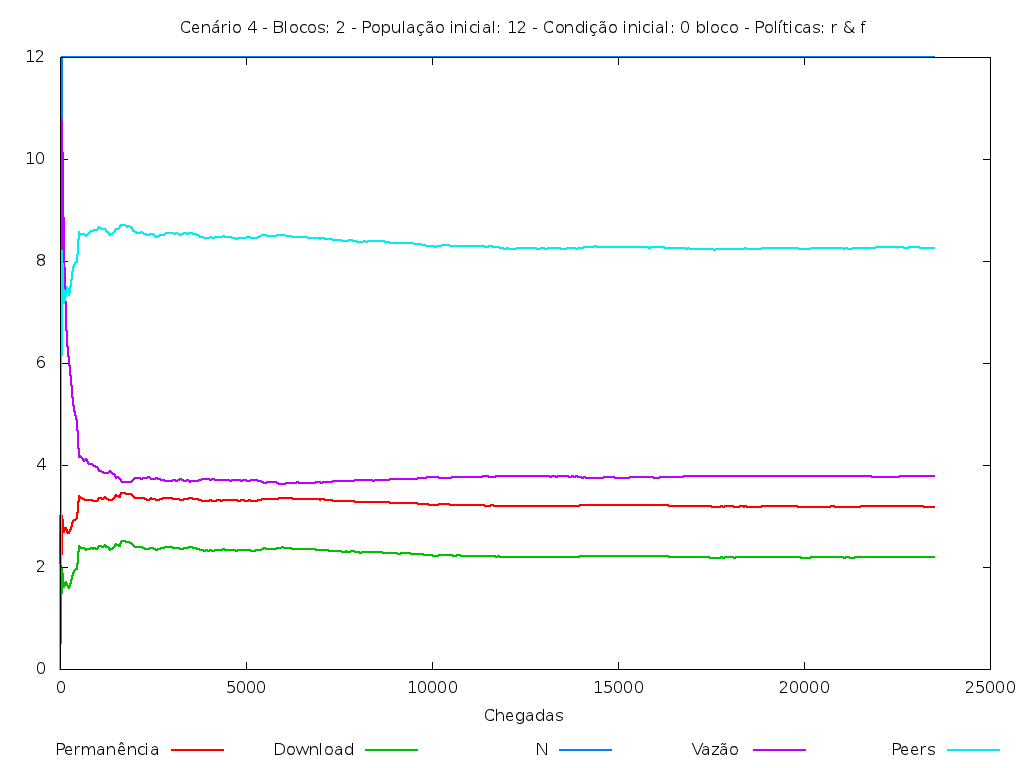
\includegraphics[scale = 0.33]{./graficos/faseTransiente/01.png}
\end{figure}

\begin{figure}
	\caption{Cenário 6 com 10 blocos e 40 pessoas}
	\label{grafTransienteCen6b10n40rr}
	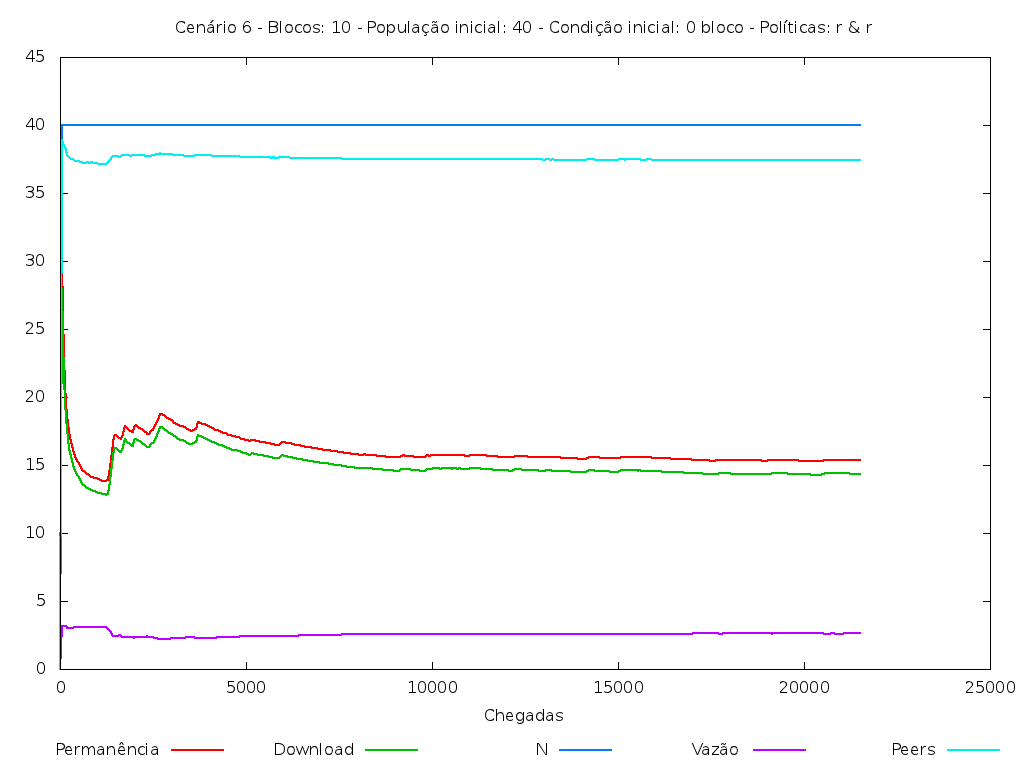
\includegraphics[scale = 0.33]{./graficos/faseTransiente/02.png}
\end{figure}

\clearpage

\begin{figure}
	\caption{Cenário 5 com 10 blocos e 43 pessoas}
	\label{grafTransienteCen5b10n43rr}
	\includegraphics[scale = 0.33]{./graficos/faseTransiente/03.png}
\end{figure}

\begin{figure}
	\caption{Cenário 1 com $\lambda = 0,9$}
	\label{grafTransienteCen1lamb0.9}
	\includegraphics[scale = 0.33]{./graficos/faseTransiente/04.png}
\end{figure}

\clearpage
\pagebreak

\subsection{Rodadas}

Para que os intervalos de confiança sejam pequenos, é preciso que cada rodada tenha um bom tamanho e que o número total de rodadas seja suficientemente grande. Inicialmente, fixamos esses números em 30 rodadas com 5000 chegadas cada, mas alguns intervalos ainda estavam grandes demais e decidimos passar a 100 rodadas.

Posteriormente, aumentamos o tamanho de cada rodada para 10000 chegadas quando buscávamos o motivo de um determinado resultado não seguir padrão que esperávamos. Mesmo tendo resolvido esta questão de outra forma, optamos por manter, no final, um total de 100 rodadas com 10000 chegadas cada.

Adicionalmente, no caso improvável de algum intervalo de confiança ser maior do que 10\%, são executadas novas rodadas até que esta condição seja satisfeita. Esta precaução mostrou-se desnecessária, visto que nenhuma simulação ultrapassou 100 rodadas.

\pagebreak

\section{Testes de Corretude}\label{TestesDeCorretude}

Para testar nossa implementação, comparamos a saída do simulador com resultados que poderíamos obter analiticamente. Desta forma, fomos capazes de concluir quando o programa estava muito próximo de estar correto.

O cenário 1 proposto na descrição do trabalho representa exatamente uma M/M/1, visto que temos o arquivo com apenas um bloco, chegadas de peers seguindo um processo Poisson e a ausência total de seeds ou chegadas por recomendação. Dado que a disciplina de atendimento não afeta a média das variáveis observadas, podemos calcular analiticamente todos os resultados e compará-los com a saída da simulação. Com isso, pudemos executar o ajuste inicial do programa.

\subsection{Dificuldades enfrentadas}

Apesar de os testes com o cenário 1 terem eliminado a maior parte de nossas dúvidas, tivemos um grande problema já no final do desenvolvimento. Ao executar as simulações, percebemos que as vazões dos cenários 4 a 6 não se comportavam exatamente como esperado.

Esta falha nos tomou vários dias para ser resolvida. Uma das causas foi não sabermos como calcular analiticamente o resultado esperado para nos certificarmos de que, de fato, havia algo errado.

Outra causa foi o efeito do erro nos resultados. O problema no código fazia com que simulássemos um cenário diferente daquele que desejávamos. Com isso, tínhamos o resultado de Little valendo para todas as variáveis e isso fez com que, novamente, ficássemos em dúvida se havia mesmo algum erro.

Terminamos por descobrir que, quando um peer chegava por recomendação, ele não transmitia nenhum dado. Desta forma, simulávamos um cenário em que um peer chegava, só recebia o arquivo do publisher e poderia ou não ficar um tempo no sistema sem fazer nada de fato. Uma vez corrigido o problema, obtivemos os dados apresentados nas próximas seções deste relatório.

\pagebreak

\section{Coleta dos dados}\label{ColetaDosDados}

\subsection{Cálculo de estimadores}

Para calcular os estimadores da média ($\hat{\mu}$) e do intervalo de confiança ($\hat{\sigma}$), são armazenados a soma das médias ($\sum_{i = 1}^n X_i$) e dos quadrados das médias ($\sum_{i = 1}^n X_ i^2$) de cada variável aleatória ao longo das rodadas. Desta forma, podemos obter ambos os estimadores.

O estimador da média vem diretamente de sua fórmula:
\begin{equation}\label{estimadorMedia}
	\hat{\mu} = {{1} \over {n}} \sum_{i = 1}^n X_i
\end{equation}

Já o estimador da variância necessita de alguma manipulação na sua fórmula orignal:
\begin{align}
	\hat{\sigma} &= {{1} \over {n - 1}} \sum_{i = 1}^n (X_i - \hat{\mu})^2 \\
	&= {{1} \over {n - 1}} \sum_{i = 1}^n (X_i^2 - 2 \hat{\mu} X_i + \mu^2) \\
	&= {{1} \over {n - 1}} \left[ \sum_{i = 1}^n X_i^2 - 2 \hat{\mu} \sum_{i = 1}^n X_i + \sum_{i = 1}^n \hat{\mu}^2 \right] \\
	&= {{1} \over {n - 1}} \left[ \sum_{i = 1}^n X_i^2 - 2 \hat{\mu} \sum_{i = 1}^n X_i + n \hat{\mu}^2 \right] \\
	&= {{1} \over {n - 1}} \left[ \sum_{i = 1}^n X_i^2 - 2 \hat{\mu} {{n}\over{n}} \sum_{i = 1}^n X_i + n \hat{\mu}^2 \right] \\
	&= {{1} \over {n - 1}} \left[ \sum_{i = 1}^n X_i^2 - n \hat{\mu}^2 \right]
\end{align}

Com isto, podemos calcular $\hat{\mu}$ e $\hat{\sigma}$ incrementalmente para qualquer variável aleatória.

\subsection{Obtenção dos intervalos de confiança}

Os intervalos de confiança foram obtidos com base na aproximação da distribuição t-Student pela distribuição normal com $n > 30$. Como pedia o enunciado, utilizamos um intervalo de confiança de 95\%. Desta forma, temos:

\begin{equation}
	P \left (\hat{\mu} - {{1,96 \hat{\sigma}} \over {\sqrt{n}}} < \mu < \hat{\mu} + {{1,96 \hat{\sigma}} \over {\sqrt{n}}} \right) \approx 0,95  ~,~~n > 30
\end{equation}
ou seja, a probabilidade de a média real estar entre os dois valores exibidos como limites do intervalo é de aproximadamente 95\%.

\section{Resultados obtidos}

\subsection{Arquivo com um bloco}

Nas figuras \ref{figPMFlamb0.1}, \ref{figPMFlamb0.5} e \ref{figPMFlamb0.9}, temos as pmfs do número de usuários no sistema para o cenário 1. Estão sobrepostos, para fins de comparação, o intervalo de confiança e o resultado analítico.

Apesar de o intervalo de confiança ser muito pequeno na maioria das vezes, podemos observar visualmente que ele engloba a média real em alguns casos. Como há muitos valores a serem exibidos quando $\lambda = 0,9$, este relatório apresenta apenas as tabelas \ref{tabPMFlamb0.1} e \ref{tabPMFlamb0.5}, que contêm, respectivamente, os valores para $\lambda = 0,1$ e $\lambda = 0,5$.

Podemos observar na tabela \ref{tabPMFlamb0.5} que, para $k = 17$, temos um valor fora do intervalo de confiança. A justificativa para isso é que trata-se de um evento raro (com probabilidade $< 4 \cdot 10^{-6}$ de ocorrer) e, portanto, a simulação sem nenhum cuidado especial com este tipo de situação pode não gerar um bom intervalo de confiança para ele. Apesar disso, podemos notar que o valor analítico está ainda bem próximo do limite superior.

Na tabela \ref{tabTempoDownloadCen1e2}, temos os tempos médios de download com seus respectivos intervalos de confiança. Em seguida temos as figuras \ref{figCDFcen1lamb0.1}, \ref{figCDFcen1lamb0.5}, \ref{figCDFcen1lamb0.9}, \ref{figCDFcen2lamb0.1}, \ref{figCDFcen2lamb0.5} e \ref{figCDFcen2lamb0.9} com os gráficos contendo a CDF do tempo de download em cada rodada para os conjuntos de parâmetros da tabela. Através das CDFs, calculamos as medianas do tempo de download, exibidas na tabela \ref{tabMedianaTempoDownload}.

Observando os resultados do parágrafo anterior, podemos concluir que a presença de usuários como seeds no sistema torna o tempo de download menor. Isto se deve ao fato de que um seed, apesar de mais lento, permitirá que mais peers sejam servidos além da capacidade do servidor.

O último cenário com apenas um bloco é o de número 3. Como trata-se de um sistema fechado, podemos avaliar a vazão como métrica de eficiência. Isto não pode ser feito nos cenários 1 e 2 porque a taxa de saída não pode ser outra que não a taxa de entrada uma vez que o sistema entre em equilíbrio. O gráfico que coloca a vazão em função do número de pessoas no sistema pode ser visto na figura \ref{vazaoCen3}. Nota-se que o sistema não é escalável, pois, sendo o publisher o único responsável por enviar o arquivo, a vazão máxima fica limitada por sua capacidade de envio.

\pagebreak

% Tabelas de pmf
\begin{center}
	\begin{table}[h]
		\caption{pmf do número de pessoas no sistema com $\lambda = 0,1$}
		\label{tabPMFlamb0.1}
		\makebox[\textwidth] 
		{
		\begin{tabular}{ | c | r | r | r | }
			\hline
			\textbf{\textit{k}} & \textbf{P(\textit{N = k}) (analítico)} & \textbf{Limite inferior} & \textbf{Limite superior} \\ \hline
			0 & 0,9 & 0,899822017190 & 0,900399632035 \\ \hline
			1 & 0,09 & 0,089602836420 & 0,090092549640 \\ \hline 
			2 & 0,009 & 0,008951846470 & 0,009130388423 \\ \hline
			3 & 0,0009 & 0,000879138968 & 0,000932046458 \\ \hline
			4 & 0,00009 & 0,000077180141 & 0,000093780926 \\ \hline
			5 & 0,000009 & 0,000005460491 & 0,000011068471 \\ \hline
			6 & 0,0000009 & 0,000000013627 & 0,000001910427 \\ \hline
			7 & 0,00000009 & 0,0\footnotemark & 0,000000164662 \\ \hline
		\end{tabular}
		}
	\end{table}
\end{center}

\begin{center}
	\begin{table}[h]
		\caption{pmf do número de pessoas no sistema com $\lambda = 0,5$}
		\label{tabPMFlamb0.5}
		\makebox[\textwidth] 
		{
		\begin{tabular}{ | c | r | r | r | }
			\hline
			\textbf{\textit{k}} & \textbf{P(\textit{N = k}) (analítico)} & \textbf{Limite inferior} & \textbf{Limite superior} \\ \hline
			0 & 0,5 & 0,497976050425 & 0,500863861786 \\ \hline
			1 & 0,25 & 0,249420542842 & 0,250861882491 \\ \hline 
			2 & 0,125 & 0,124654767781 & 0,125790005825 \\ \hline
			3 & 0,0625 & 0,062187016865 & 0,063157683324 \\ \hline
			4 & 0,03125 & 0,030623810927 & 0,031492326347 \\ \hline
			5 & 0,015625 & 0,015384256463 & 0,016031342774 \\ \hline
			6 & 0,0078125 & 0,007638869747 & 0,008123794203 \\ \hline
			7 & 0,00390625 & 0,003668546214 & 0,003983212940 \\ \hline
			8 & 0,001953125 & 0,001869532721 & 0,002092272616 \\ \hline
			9 & 0,0009765625 & 0,000935911990 & 0,001100733438 \\ \hline
			10 & 0,00048828125 & 0,000461616564 & 0,000582360346 \\ \hline
			11 & 0,000244140625 & 0,000231226212 & 0,000321205960 \\ \hline
			12 & 0,000122070312 & 0,000114439879 & 0,000169397027 \\ \hline
			13 & 0,000061035156 & 0,000049574184 & 0,000091966384 \\ \hline
			14 & 0,000030517578 & 0,000025214314 & 0,000054621483 \\ \hline
			15 & 0,000015258789 & 0,000006174981 & 0,000019933314 \\ \hline
			16 & 0,000007629395 & 0,000000902206 & 0,000012079891 \\ \hline
			17 & 0,000003814697 & 0,0\footnotemark[\value{footnote}] & 0,000003125728 \\ \hline
			18 & 0,000001907349 & 0,0\footnotemark[\value{footnote}] & 0,000000273893 \\ \hline
		\end{tabular}
		}
	\end{table}
\end{center}

\footnotetext{O limite inferior calculado aqui tem valor negativo, mas, uma vez que probabilidades são necessariamente não negativas, podemos alterá-lo para 0 sem modificar a probabilidade do intervalo. Temos $P(\mu \in [L, U]) = 0,95$ e $P(\mu \in [L, 0)) = 0$, o que significa que $P(\mu \notin [L, 0)) = 1$. Como $[L, 0) \subset [L, U]$, $P(\mu \in [L, U], \mu \in [L, 0)) = P(\mu \in [L, U])$. Logo, $P(\mu \in [0, U] \mid \mu \notin [L, 0)) = {{P(\mu \in [L, U])} \over {P(\mu \notin [L, 0))}} = 0,95$.}

\clearpage
\pagebreak

% Gráficos de pmf
\begin{figure}
	\caption{pmf do número de pessoas no sistema com $\lambda = 0,1$}
	\label{figPMFlamb0.1}
	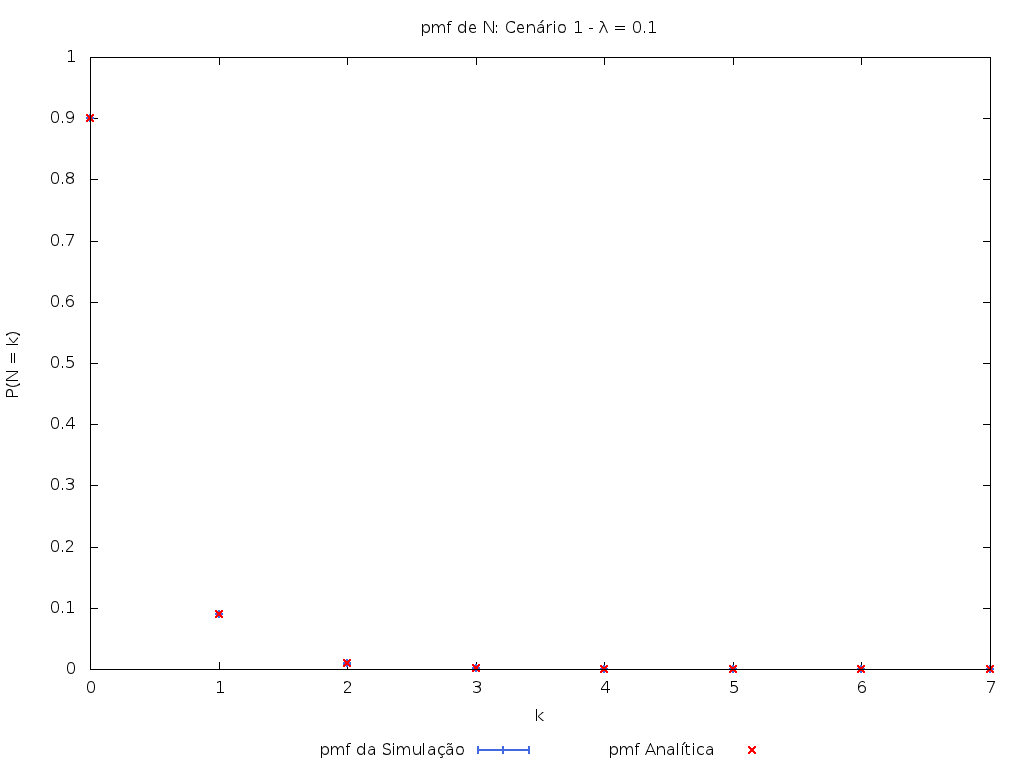
\includegraphics[scale = 0.33]{./graficos/pmf/01.png}
\end{figure}

\begin{figure}
	\caption{pmf do número de pessoas no sistema com $\lambda = 0,5$}
	\label{figPMFlamb0.5}
	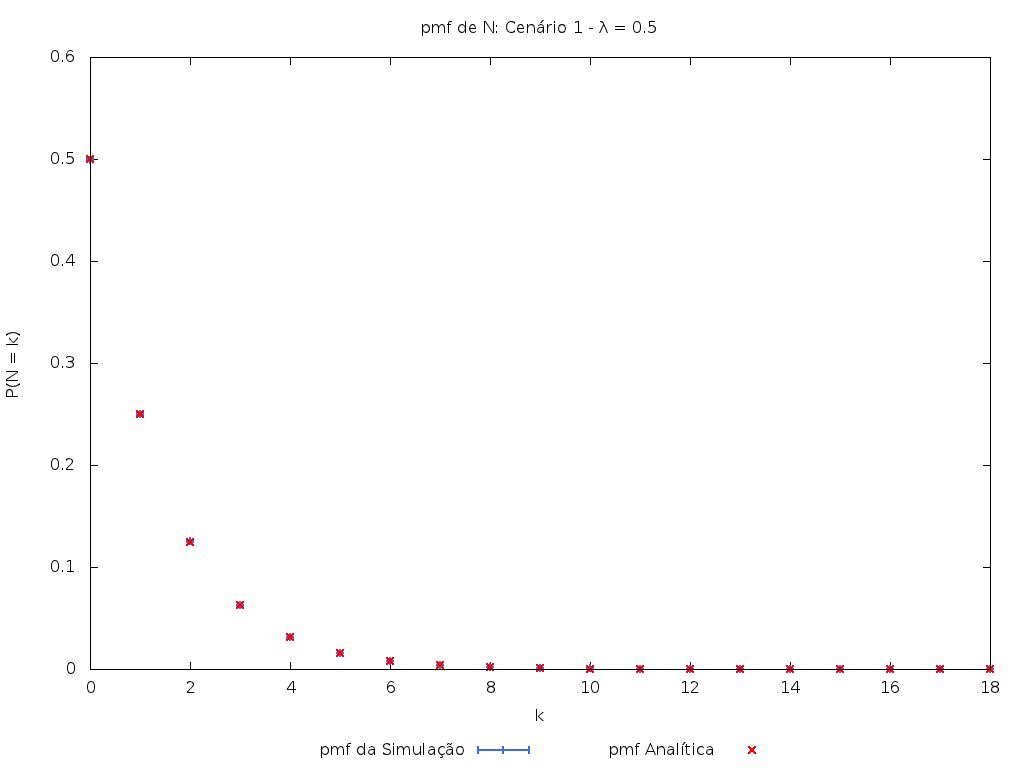
\includegraphics[scale = 0.33]{./graficos/pmf/02.png}
\end{figure}

\clearpage
\pagebreak

\begin{figure}
	\caption{pmf do número de pessoas no sistema com $\lambda = 0,9$}
	\label{figPMFlamb0.9}
	\includegraphics[scale = 0.33]{./graficos/pmf/03.png}
\end{figure}

% Tabela do tempo de download
\begin{center}
	\begin{table}[h]
		\caption{Média do tempo de download nos cenários 1 e 2}
		\label{tabTempoDownloadCen1e2}
		\makebox[\textwidth] 
		{
		\begin{tabular}{ | c | c | c | p{2.5cm} | p{3cm} | p{3cm} | }
		\hline
		$\boldsymbol\lambda$ & $\boldsymbol\mu$ & $\boldsymbol\gamma$ & \textbf{Tempo médio de download} & \textbf{Limite inferior do intervalo de confiança} & \textbf{Limite superior do intervalo de confiança} \\ \hline \hline
		0,1 & - & $\infty$ & 1,109913531662 & 1,107213957314 & 1,112613106010 \\ \hline
		0,5 & - & $\infty$ & 2,002085122497 & 1,991433307156 & 2,012736937837 \\ \hline
		0,9 & - & $\infty$ & 10,135659151670 & 9,749186384809 & 10,522131918532 \\ \hline
		0,1 & 0,1 & 0,1 & 1,006295891166 & 1,003802169978 & 1,008789612354 \\ \hline
		0,5 & 0,1 & 0,1 & 1,046063420675 & 1,041709828877 & 1,050417012473 \\ \hline
		0,9 & 0,1 & 0,1 & 1,085723681141 & 1,079771062357 & 1,091676299925 \\ \hline
		\end{tabular}
		}
	\end{table}
\end{center}

\clearpage
\pagebreak

%Gráficos de CDF do tempo de download
\begin{figure}
	\caption{CDF do tempo de download no cenário1  com $\lambda = 0.1$}
	\label{figCDFcen1lamb0.1}
	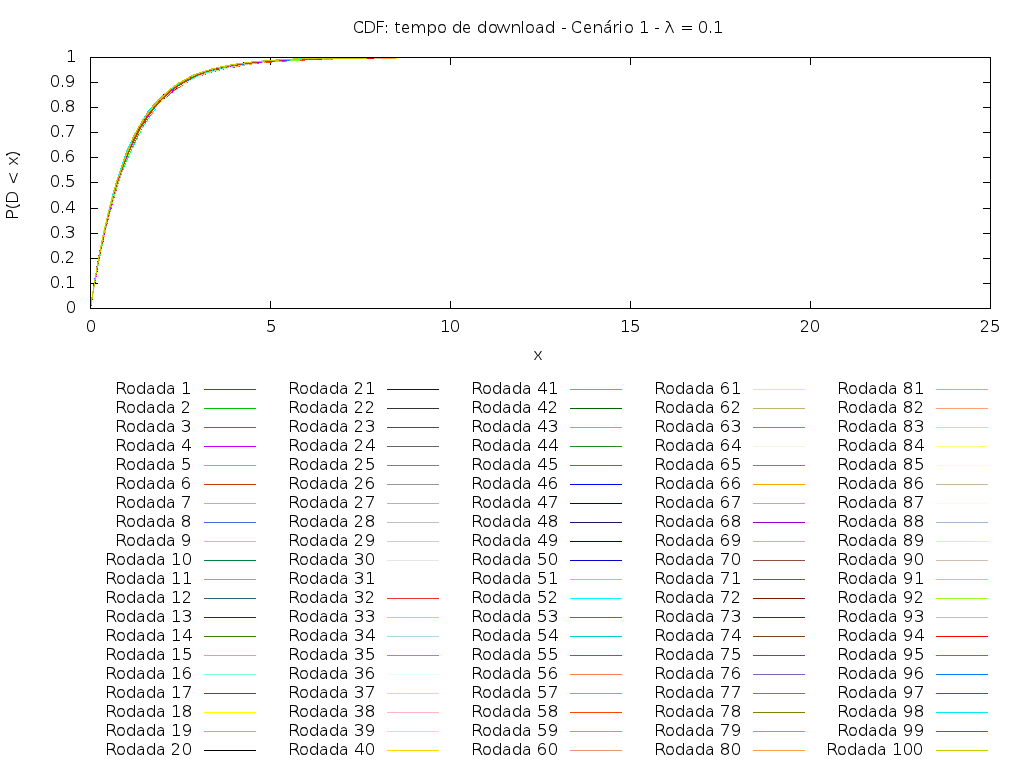
\includegraphics[scale = 0.33]{./graficos/cdf/01.png}
\end{figure}

\begin{figure}
	\caption{CDF do tempo de download no cenário 1 com $\lambda = 0.5$}
	\label{figCDFcen1lamb0.5}
	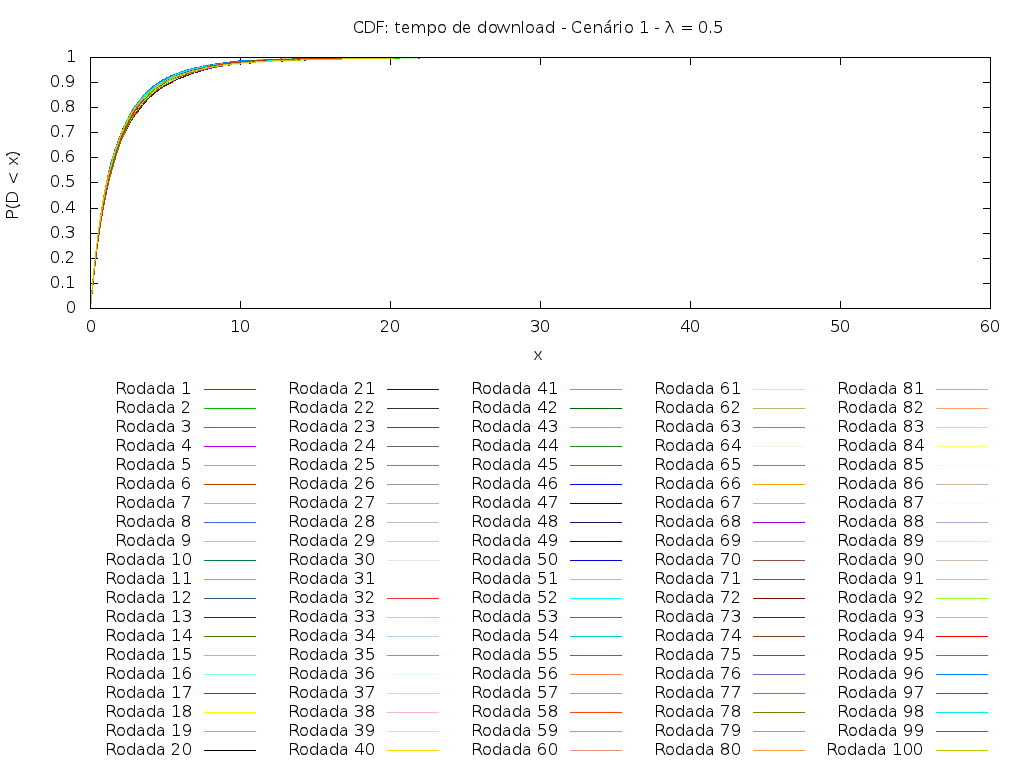
\includegraphics[scale = 0.33]{./graficos/cdf/02.png}
\end{figure}

\clearpage
\pagebreak

\begin{figure}
	\caption{CDF do tempo de download no cenário 1 com $\lambda = 0.9$}
	\label{figCDFcen1lamb0.9}
	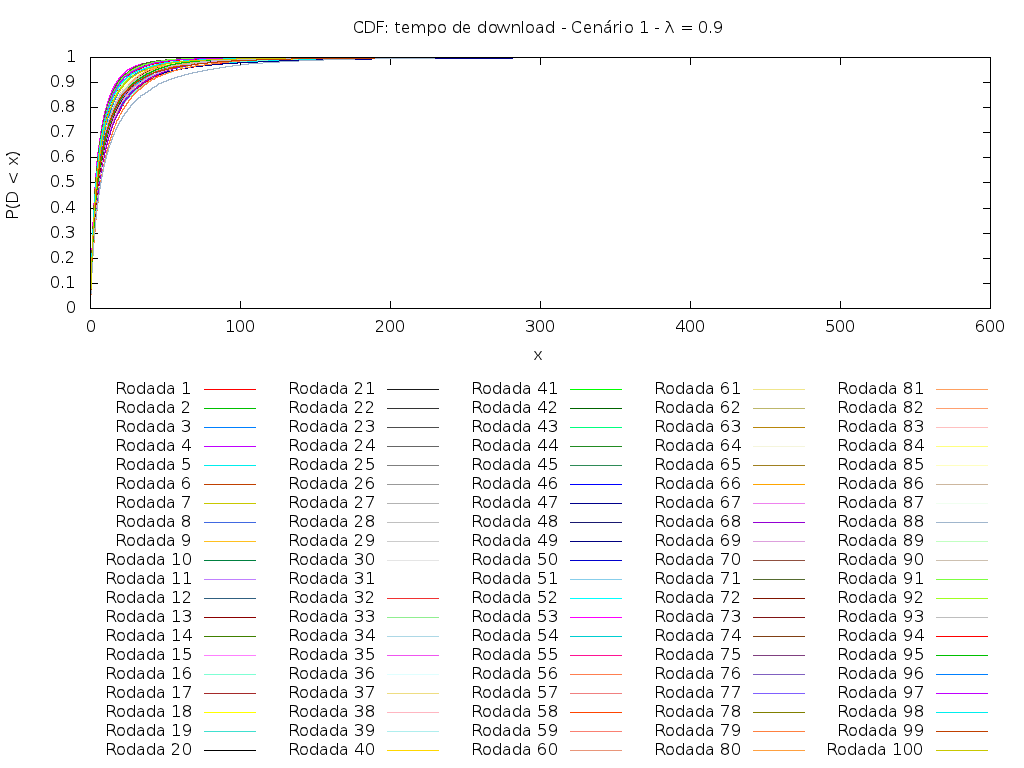
\includegraphics[scale = 0.33]{./graficos/cdf/03.png}
\end{figure}

\begin{figure}
	\caption{CDF do tempo de download no cenário 2 com $\lambda = 0.1$}
	\label{figCDFcen2lamb0.1}
	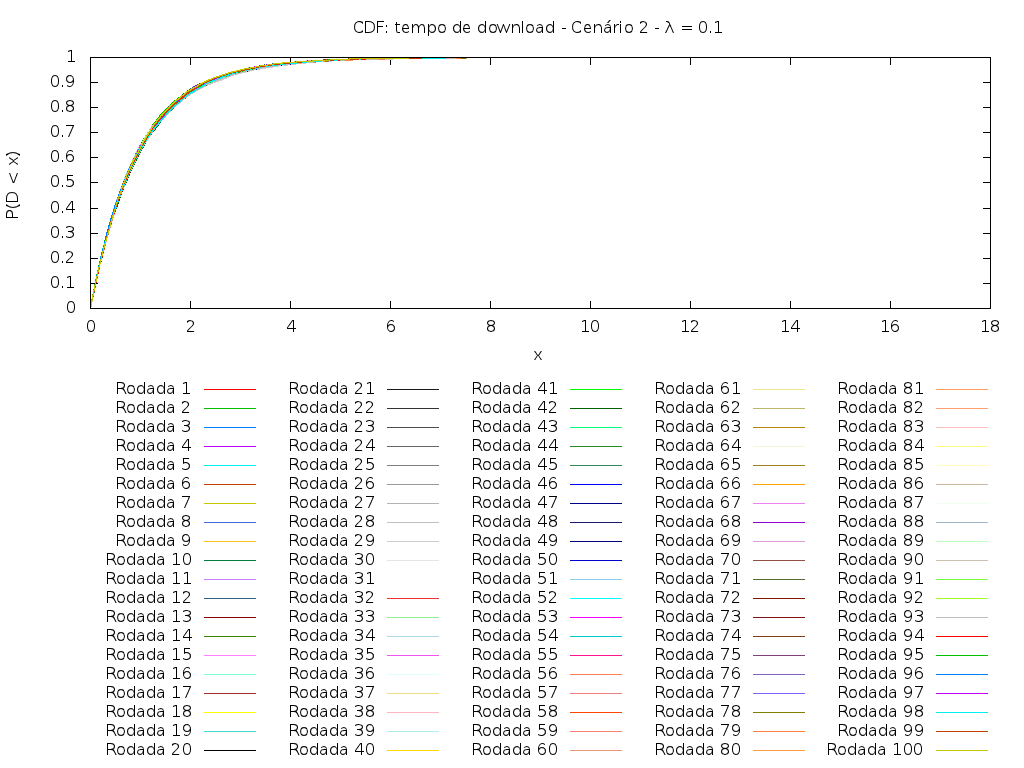
\includegraphics[scale = 0.33]{./graficos/cdf/04.png}
\end{figure}

\clearpage
\pagebreak

\begin{figure}
	\caption{CDF do tempo de download no cenário 2 com $\lambda = 0.5$}
	\label{figCDFcen2lamb0.5}
	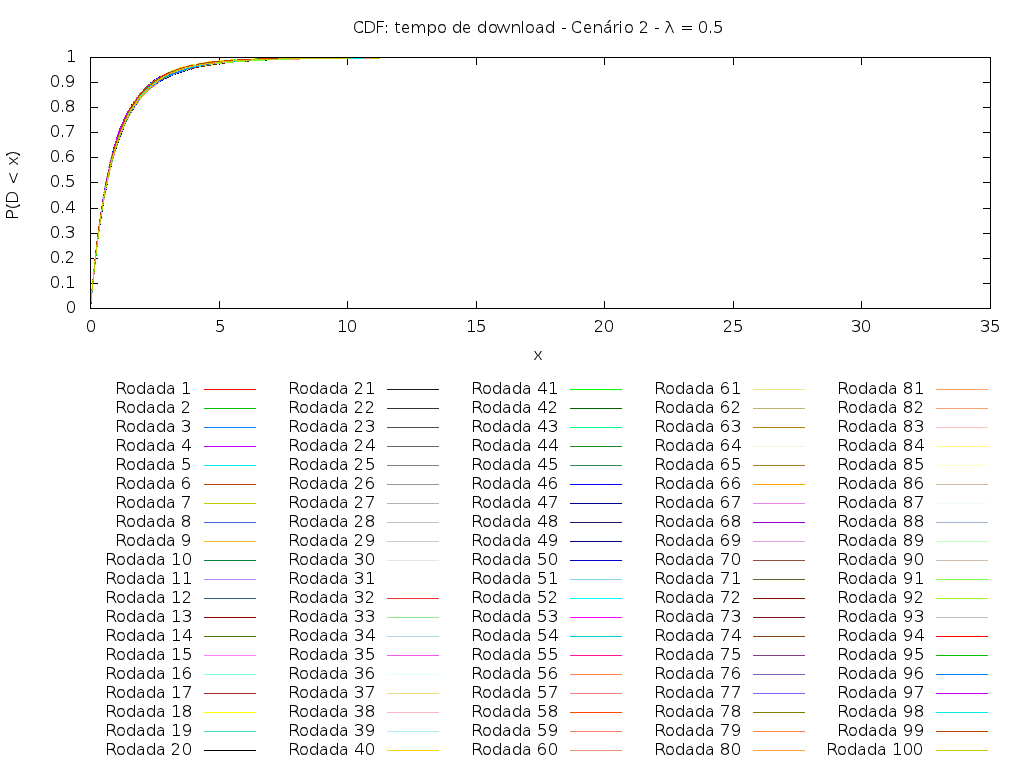
\includegraphics[scale = 0.33]{./graficos/cdf/05.png}
\end{figure}

\begin{figure}
	\caption{CDF do tempo de download no cenário 2 com $\lambda = 0.9$}
	\label{figCDFcen2lamb0.9}
	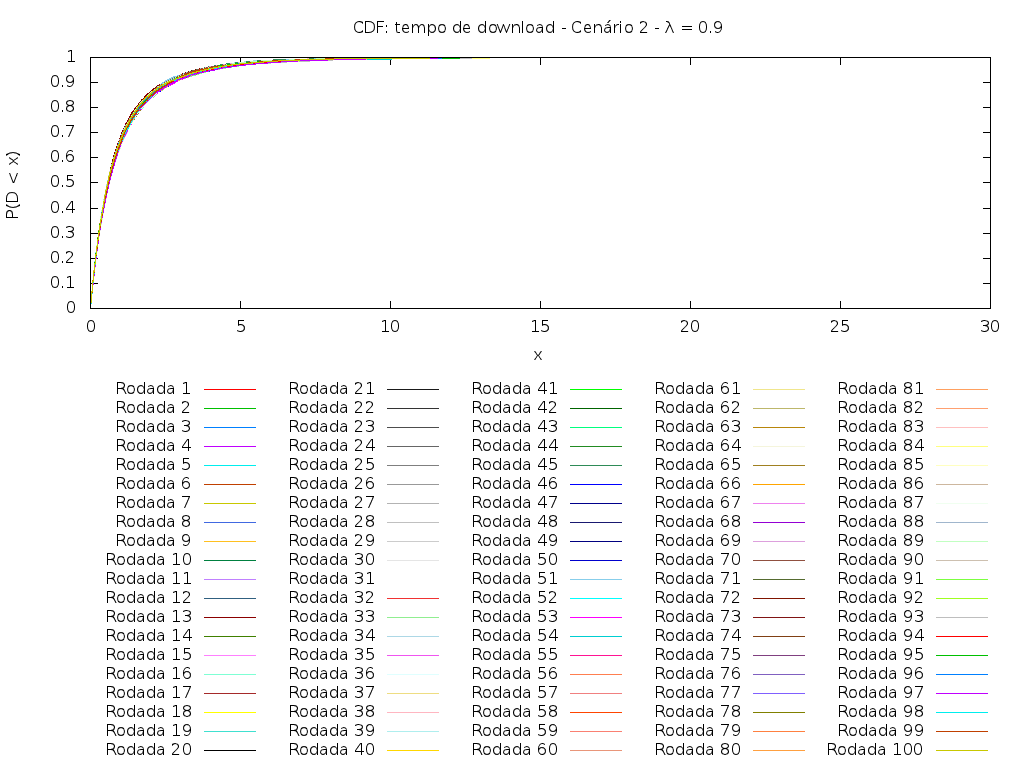
\includegraphics[scale = 0.33]{./graficos/cdf/06.png}
\end{figure}

\clearpage
\pagebreak

\begin{center}
	\begin{table}[h]
		\caption{Mediana do tempo de download com intervalo de confiança de 95\%}
		\label{tabMedianaTempoDownload}
		\makebox[\textwidth] 
		{
		\begin{tabular}{ | c | c | c | p{2.5cm} | p{3cm} | p{3cm} | }
		\hline
		$\boldsymbol\lambda$ & $\boldsymbol\mu$ & $\boldsymbol\gamma$ & \textbf{Mediana do tempo de download} & \textbf{Limite inferior do intervalo de confiança} & \textbf{Limite superior do intervalo de confiança} \\ \hline \hline
		0,1 & - & $\infty$ & 0,737047408215 & 0,722433655393 & 0,751661161036 \\ \hline
		0,5 & - & $\infty$ & 1,124063814379 & 1,101496212869 & 1,146631415889 \\ \hline
		0,9 & - & $\infty$ & 4,405159232804 & 4,245628264486 & 4,564690201122 \\ \hline
		0,1 & 0,1 & 0,1 & 0,667048594407 & 0,653845586561 & 0,680251602253 \\ \hline
		0,5 & 0,1 & 0,1 & 0,616956850412 & 0,604620695764 & 0,629293005060 \\ \hline
		0,9 & 0,1 & 0,1 & 0,585914289199 & 0,574149924840 & 0,597678653559 \\ \hline
		\end{tabular}
		}
	\end{table}
\end{center}

\vspace{3cm}

\begin{figure}[h]
	\caption{Vazão do cenário 3}
	\label{vazaoCen3}
	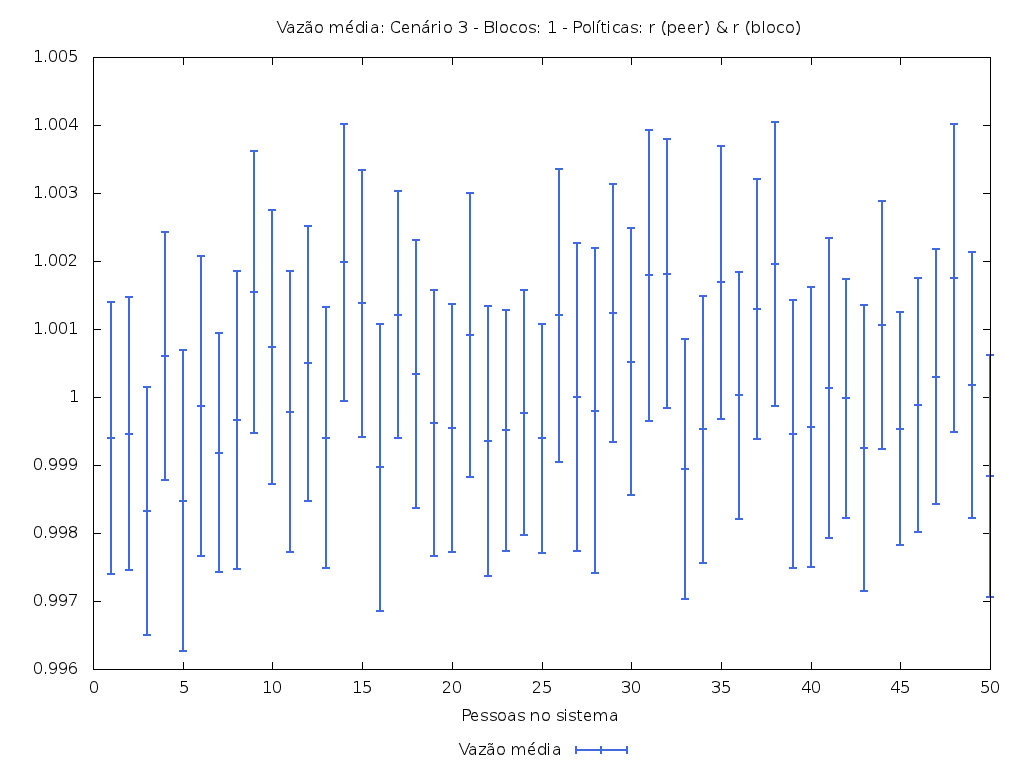
\includegraphics[scale = 0.33]{./graficos/vazaoCen3/01.png}
\end{figure}

\clearpage
\pagebreak

\subsection{Arquivo com dois blocos}

\subsubsection{\textit{Random peer / Random useful piece}}

Nas figuras \ref{vazao4b2rr}, \ref{vazao5b2rr} e \ref{vazao6b2rr} podemos ver a evolução da vazão com o aumento do número de pessoas no sistema, respectivamente, nos cenários 4, 5 e 6 com seus intervalos de confiança de 95\%.

Comparando as curvas correspondentes aos cenários 4 e 5, podemos observar que a presença de seeds influencia a escalabilidade do sistema, mesmo os peers transmitindo blocos entre si. No primeiro cenário, podemos ver que a vazão cresce com o número de usuários até o limite desta simulação, enquanto no cenário 5 o ela estabiliza em torno de 1 saída por unidade de tempo. É notável o fato de que isto acontece mesmo que, em razão do seu tempo de permanência no sistema, a média seja de apenas 1 transmissão por seed.

\begin{proof}

Sejam $K$ o número de transmissões de um seed e $X$ o tempo de permanência do mesmo após terminar o download. Sabemos que

\begin{equation}\label{esperancaTransformada}
	E[K] =\left. K'(z) \right |_{z = 1}
\end{equation}
e também que

\begin{equation}\label{transZtransLaplace}
	K(z) = X^*(\mu - \mu z) = {{\gamma} \over {\gamma + (\mu - \mu z)}}
\end{equation}

Unindo as equações \ref{esperancaTransformada} e \ref{transZtransLaplace}, temos

\begin{align}
	E[K] &= \left. K'(z) \right |_{z = 1} \\
	&= {{\gamma \mu} \over {(\gamma - \mu + \mu)^2}} \\
	&= {{\mu} \over {\gamma}} \\
	&= 1 \text{ transmissão por seed.}
\end{align}
\end{proof}

Observando, agora, as curvas obtidas para os cenários 4 e 6, que reduzir a capacidade de serviço do publisher diminui a vazão do sistema, mas que o efeito desta mudança não é tão acentuado quanto se esperaria caso todas as tranmissões dependessem dele. Uma redução da taxa de envio do publisher à metade levou a vazão a uma redução de aproximadamente 33\% para 25 pessoas presentes no sistema e de cerca de 25\% para 50 pessoas.

À medida em que aumentamos o número de pessoas presentes, é esperado que a capacidade de serviço do publisher tenha cada vez menos influência. Isto porque, com mais pessoas, temos um maior fluxo de dados entre os próprios usuários e o publisher fica responsável por uma fração cada vez menor do tráfego. Desta forma, a diferença entre os cenários 4 e 6 tende a diminuir cada vez mais caso simulemos cenários ainda maiores.

\pagebreak

\begin{figure}
	\caption{\textit{Random peer / Random useful piece} - Vazão por quantidade de pessoas no cenário 4}
	\label{vazao4b2rr}
	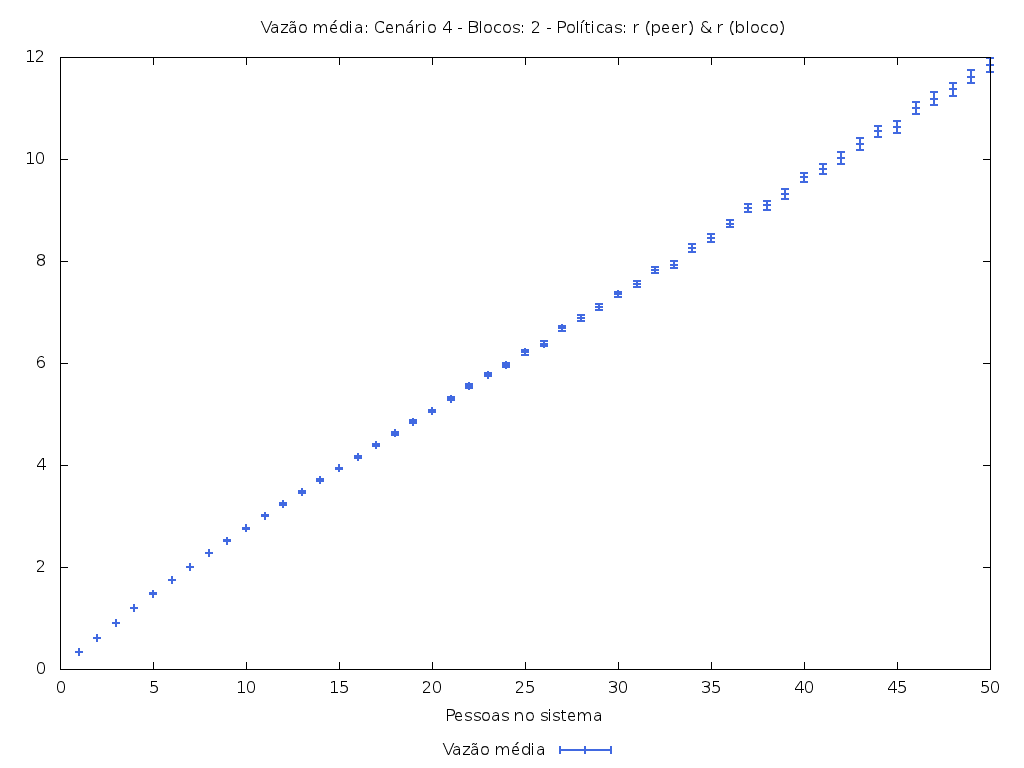
\includegraphics[scale = 0.33]{./graficos/2blocosRR/01.png}
\end{figure}

\begin{figure}
	\caption{\textit{Random peer / Random useful piece} - Vazão por quantidade de pessoas no cenário 5}
	\label{vazao5b2rr}
	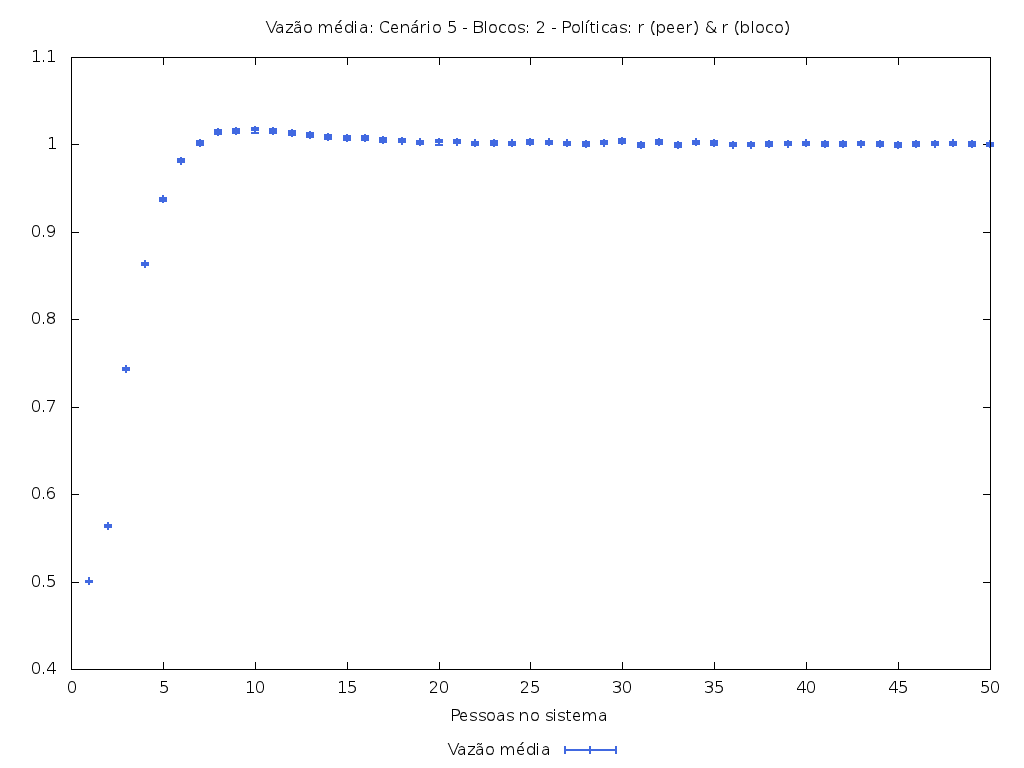
\includegraphics[scale = 0.33]{./graficos/2blocosRR/02.png}
\end{figure}

\clearpage
\pagebreak

\begin{figure}
	\caption{\textit{Random peer / Random useful piece} - Vazão por quantidade de pessoas no cenário 6}
	\label{vazao6b2rr}
	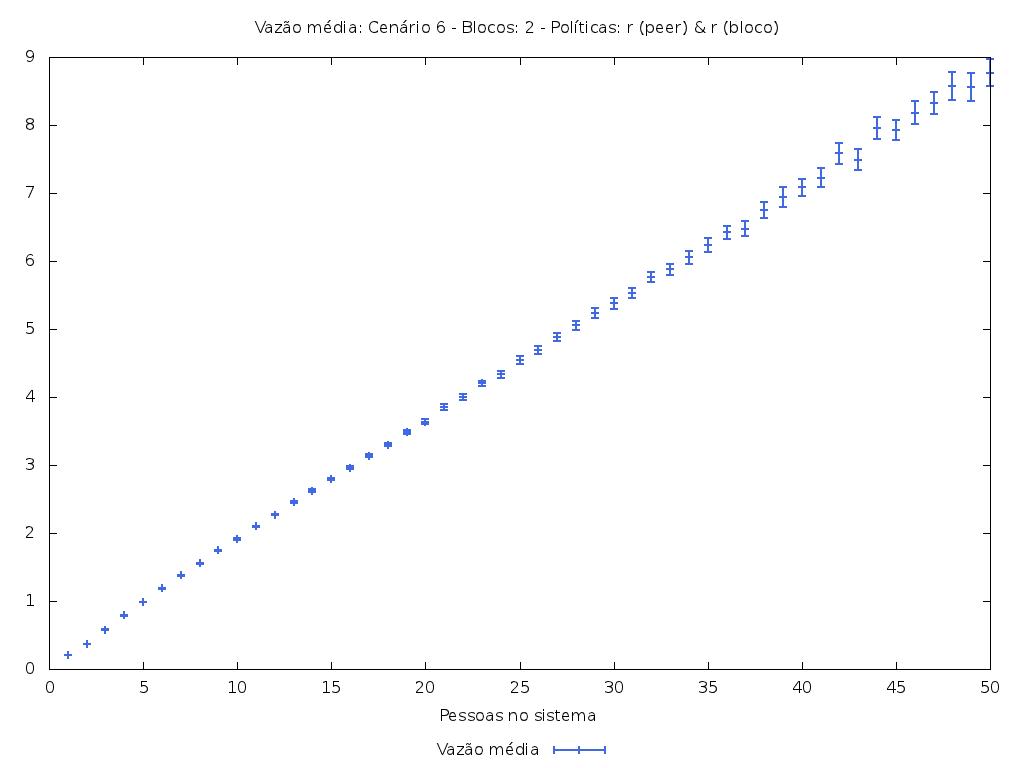
\includegraphics[scale = 0.33]{./graficos/2blocosRR/03.png}
\end{figure}

\pagebreak

\subsubsection{\textit{Random peer / Rarest first piece}}

Nas figuras \ref{vazao4b2rf}, \ref{vazao5b2rf} e \ref{vazao6b2rf} podemos ver a evolução da vazão com o aumento do número de pessoas no sistema, respectivamente, nos cenários 4, 5 e 6 com seus intervalos de confiança de 95\%.

Nos cenários 4 e 6 é possível notar um aumento efetivo na vazão. Já no cenário 5, ela parece aumentar bem, até que regride e torna a se aproximar do mesmo valor de 1 saída por unidade de tempo ao redor do qual estabilizou-se no cenário de mesmo número com a política \textit{Random peer / Random useful piece}. A melhora observada na presença de seeds deve-se ao fato de que o envio do bloco mais raro faz com que os blocos mais comuns possem a ser enviados pelos outros peers. Com isso, há um melhor direcionamento da capacidade de serviço do publisher e dos seeds e um melhor aproveitamento das transmissões entre peers. No cenário 5, o publisher ainda é responsável por suprir a maior parte da demanda por blocos mais raros e, assim, não é possível um aumento real da vazão deste sistema.

Com esta nova política, a diminuição da capacidade de serviço do publisher teve um efeito ainda menor sobre o sistema como um todo, como podemos perceber ao notar a vazão muito próxima nos cenários 4 e 6. Entendemos que isto se deve ao fato de que, agora, as transmissões entre peers passam a ser mais efecientes, sendo o publisher e os seeds responsáveis apenas por evitar que um determinado bloco não esteja mais presente no sistema. Isso faz com que uma maior quantidade de transmissões entre peers tenha sucesso, o que equilibra os dois cenários, visto que estes diferenciam-se apenas pela taxa de upload do publisher.

\pagebreak

\begin{figure}
	\caption{\textit{Random peer /  Rarest first piece} - Vazão por quantidade de pessoas no cenário 4}
	\label{vazao4b2rf}
	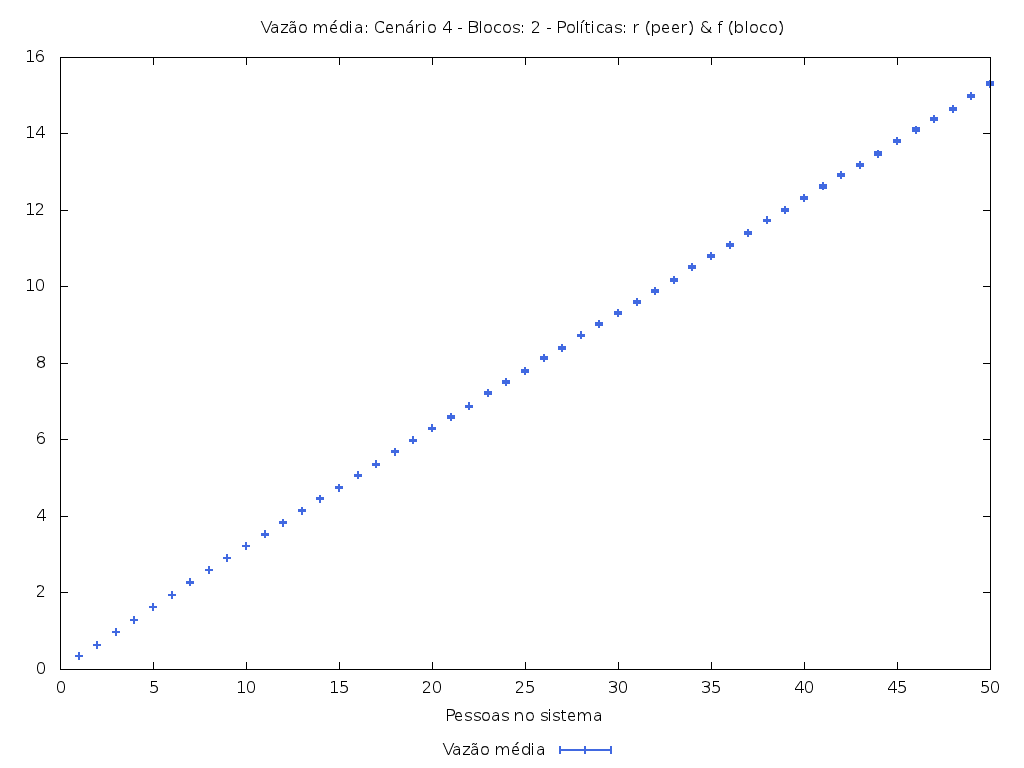
\includegraphics[scale = 0.33]{./graficos/2blocosRF/01.png}
\end{figure}

\begin{figure}
	\caption{\textit{Random peer /  Rarest first piece} - Vazão por quantidade de pessoas no cenário 5}
	\label{vazao5b2rf}
	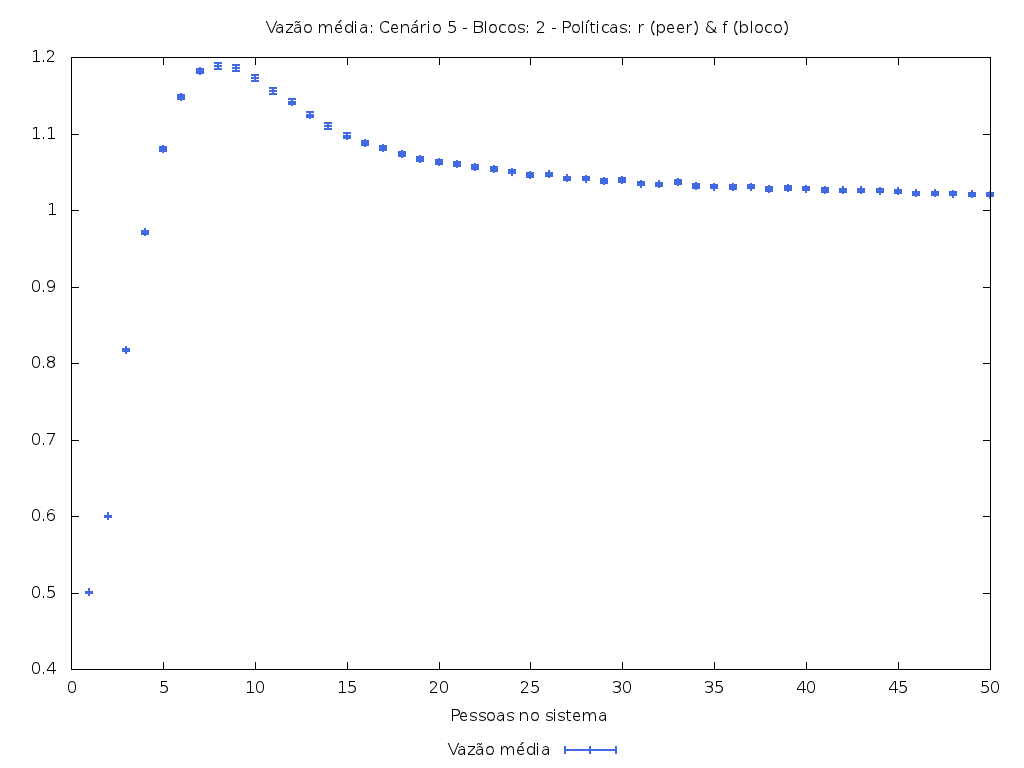
\includegraphics[scale = 0.33]{./graficos/2blocosRF/02.png}
\end{figure}

\clearpage
\pagebreak

\begin{figure}
	\caption{\textit{Random peer /  Rarest first piece} - Vazão por quantidade de pessoas no cenário 6}
	\label{vazao6b2rf}
	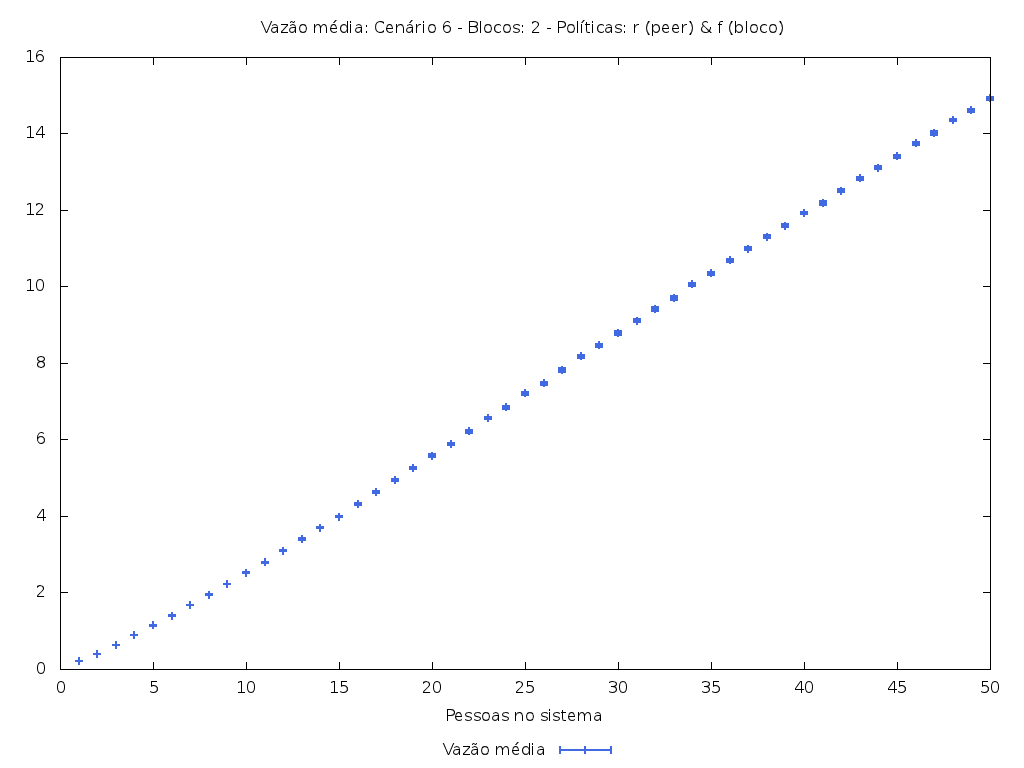
\includegraphics[scale = 0.33]{./graficos/2blocosRF/03.png}
\end{figure}

\pagebreak

\subsubsection{Arquivo com 10 blocos}

Nas figuras \ref{vazao4b10}, \ref{vazao5b10} e \ref{vazao6b10} podemos ver a evolução da vazão com o aumento do número de pessoas no sistema, respectivamente, nos cenários 4, 5 e 6 com seus intervalos de confiança de 95\%. Para os cenários com 10 blocos, foi utilizada a política \textit{Random peer / Random useful piece}.

Com o aumento no número de blocos, as tendências observadas em cada cenário com dois blocos mantiveram-se, isto é, os cenários 4 e 6 apresentaram crescimento, enquanto no cenário 5, a partir de uma determinada quantidade de pessoas presentes no sistema, a vazão tendeu a estabilizar-se. Essas comparações com as situações em que havia apenas 2 blocos, no entanto, devem parar por aqui, pois ir além disso não representaria a realidade. Uma vez que a taxa de upload destas simulações é dada em blocos por segundo, temos, na realidade, arquivos 5 vezes maiores.

Apesar disso, é notável o fato de que a vazão do cenário 5 aumentou, mesmo que os arquivos tenham tornado-se muito maiores. Isto, acreditamos, deve-se ao fato de que os peers devem esperar receber todos os 10 blocos para concluir o download, ou seja, precisam continuar no sistema enquanto possuem uma quantidade maior de blocos e têm, assim, uma maior chance de aproveitar suas tentativas de transmissão. O tempo de download não aumenta, visto que isso iria de encontro ao resultado de Little, mas há uma maior chance de não se desperdiçar uma tentativa de envio de um bloco.

A vantagem de haver seeds no sistema ainda é evidente. A vazão, nos cenários 4 e 6, apresenta a mesma tendência de crescimento contínuo, enquanto, no cenário 5 continua tendendo a estabilizar-se ao redor de um valor fixo.

Já a redução da capacidade de serviço do publisher teve um efeito menos acentuado do que o que pode ser observado nas figuras \ref{vazao4b2rr} e \ref{vazao6b2rr}. Isto ocorre pelo mesmo motivo que a vazão do sistema aumentou para o cenário 5, que é a maior influência dos peers no envio do arquivo, assim como quando alteramos a política de seleção de bloco para \textit{Rarest first piece}.

\vspace{3cm}

\begin{figure}[h]
	\caption{Arquivo com 10 blocos - Vazão por quantidade de pessoas no cenário 4}
	\label{vazao4b10}
	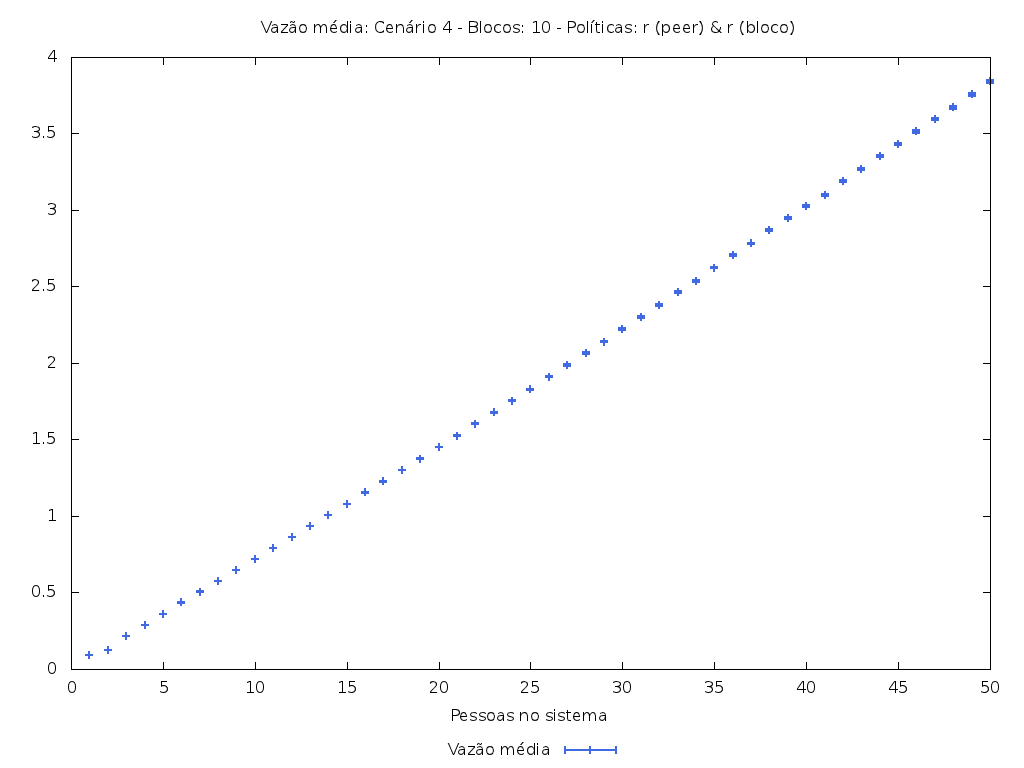
\includegraphics[scale = 0.33]{./graficos/10blocos/01.png}
\end{figure}

\clearpage
\pagebreak

\begin{figure}
	\caption{Arquivo com 10 blocos - Vazão por quantidade de pessoas no cenário 5}
	\label{vazao5b10}
	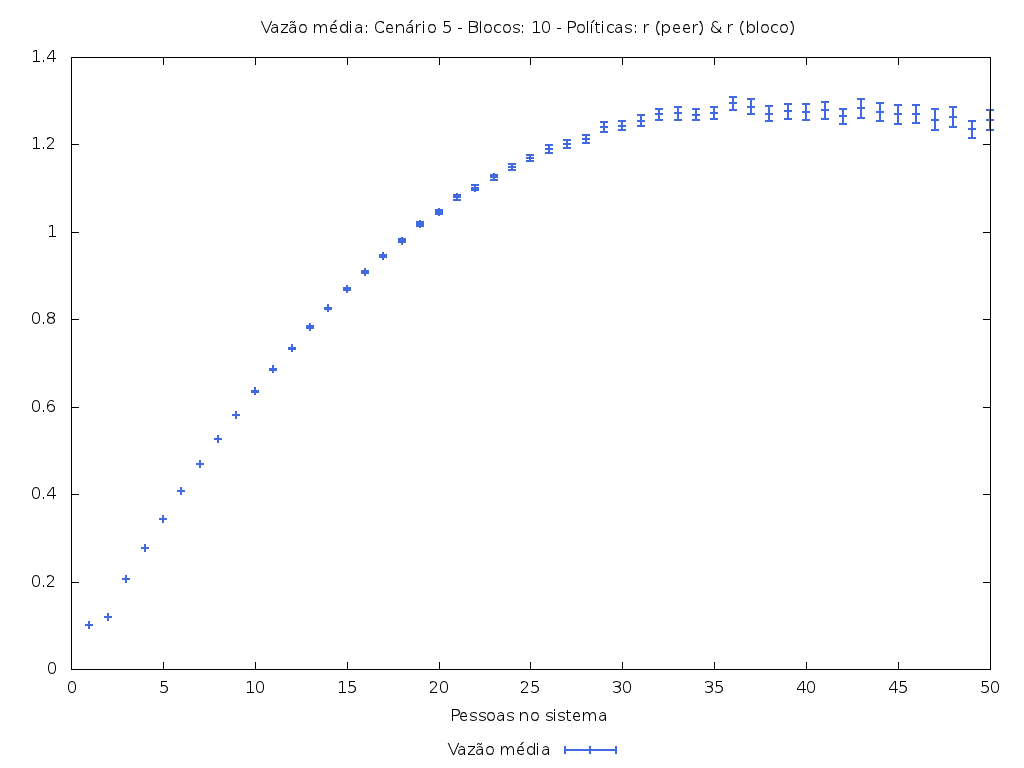
\includegraphics[scale = 0.33]{./graficos/10blocos/02.png}
\end{figure}

\begin{figure}
	\caption{Arquivo com 10 blocos - Vazão por quantidade de pessoas no cenário 6}
	\label{vazao6b10}
	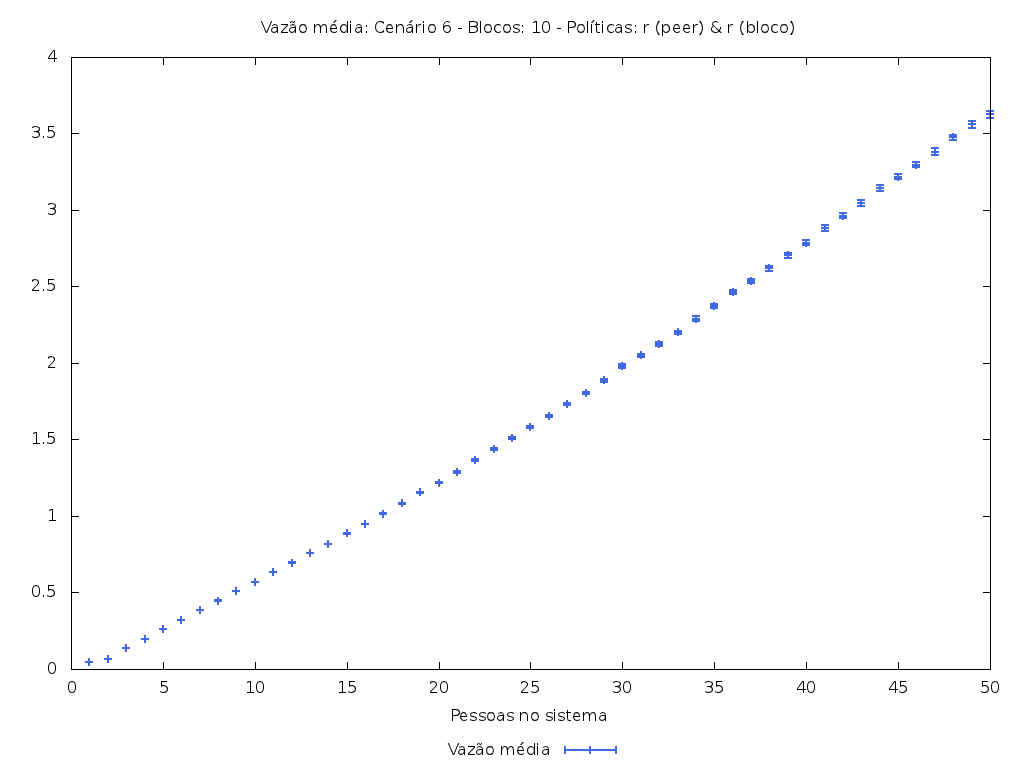
\includegraphics[scale = 0.33]{./graficos/10blocos/03.png}
\end{figure}

\clearpage
\pagebreak

\subsection{Variando as condições iniciais}

Simulamos o cenário 5, no caso em que a população inicial era de 50 pessoas, sob as seguintes condições:
\begin{enumerate}
	\item Política \textit{Random peer / Random useful piece} e todos os peers iniciando sem nenhum bloco;
	\item Política \textit{Random peer / Random useful piece} e todos os peers iniciando com 1 bloco;
	\item Política \textit{Random peer / Rarest first piece} e todos os peers iniciando sem nenhum bloco;
	\item Política \textit{Random peer / Rarest first piece} e todos os peers iniciando com 1 bloco.
\end{enumerate}

Pode-se ver um exemplo de simulação em cada uma das figuras \ref{figCI0rr}, \ref{figCI1rr}, \ref{figCI0rf} e \ref{figCI1rf}, mas, ao todo, executamos 30 vezes cada um dos itens. Obtivemos, ao final, os resultados exibidos na tabela \ref{tabCItrans} com um intervalo de confiança de 95\%. A numeração das configurações refere-se aos itens acima.

\begin{center}
	\begin{table}[h]
		\caption{Duração da fase transiente com alteração da condição inicial em número de chegadas}
		\label{tabCItrans}
		\makebox[\textwidth] 
		{
		\begin{tabular}{ | c | c | c | c |  }
		\hline
		\textbf{Configuração} & \textbf{Média} & \textbf{Limite inferior} & \textbf{Limite Superior} \\ \hline
		1 & 6283,33333333 & 5784,55073878 & 6782,11592789 \\ \hline
		2 & 6533,33333333 & 5939,10830275 & 7127,55836392 \\ \hline
		3 & 6566,66666667 & 6252,40089828 & 6880,93243505 \\ \hline
		4 & 6316,66666667 & 5911,14786079 & 6722,18547254 \\ \hline
		\end{tabular}
		}
	\end{table}
\end{center}

Com base nos dados da tabela, não podemos afirmar que existe, de fato, alguma diferença entre as durações das fases transientes.

\pagebreak

\begin{figure}
	\caption{Visualização da fase transiente com política \textit{Random peer / Random useful piece} e todos os peers iniciando sem nenhum bloco}
	\label{figCI0rr}
	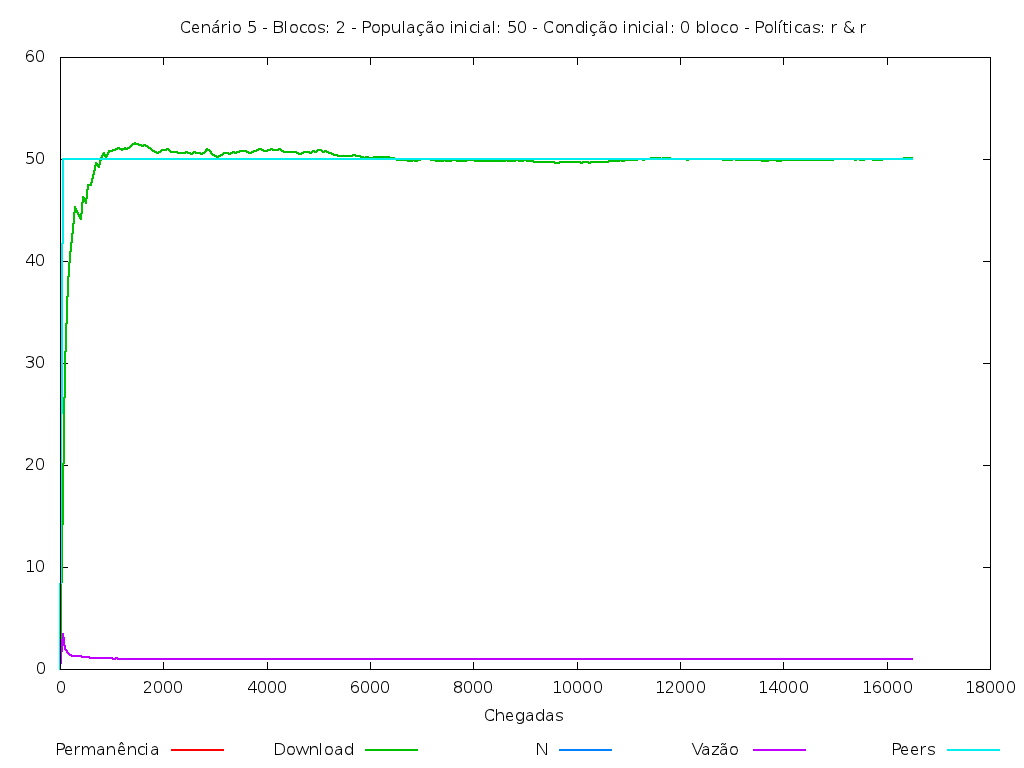
\includegraphics[scale = 0.33]{./graficos/condicaoInicial/01.png}
\end{figure}

\begin{figure}
	\caption{Visualização da fase transiente com política \textit{Random peer / Random useful piece} e todos os peers iniciando com 1 bloco}
	\label{figCI1rr}
	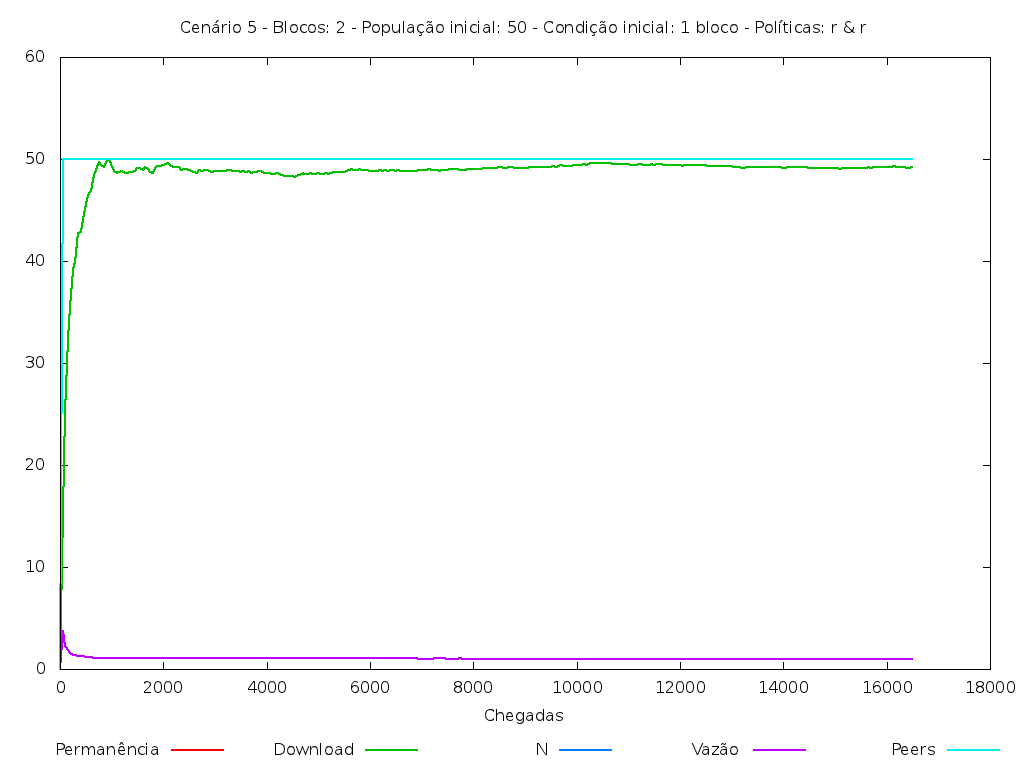
\includegraphics[scale = 0.33]{./graficos/condicaoInicial/02.png}
\end{figure}

\clearpage
\pagebreak

\begin{figure}
	\caption{Visualização da fase transiente com política \textit{Random peer / Rarest first piece} e todos os peers iniciando sem nenhum bloco}
	\label{figCI0rf}
	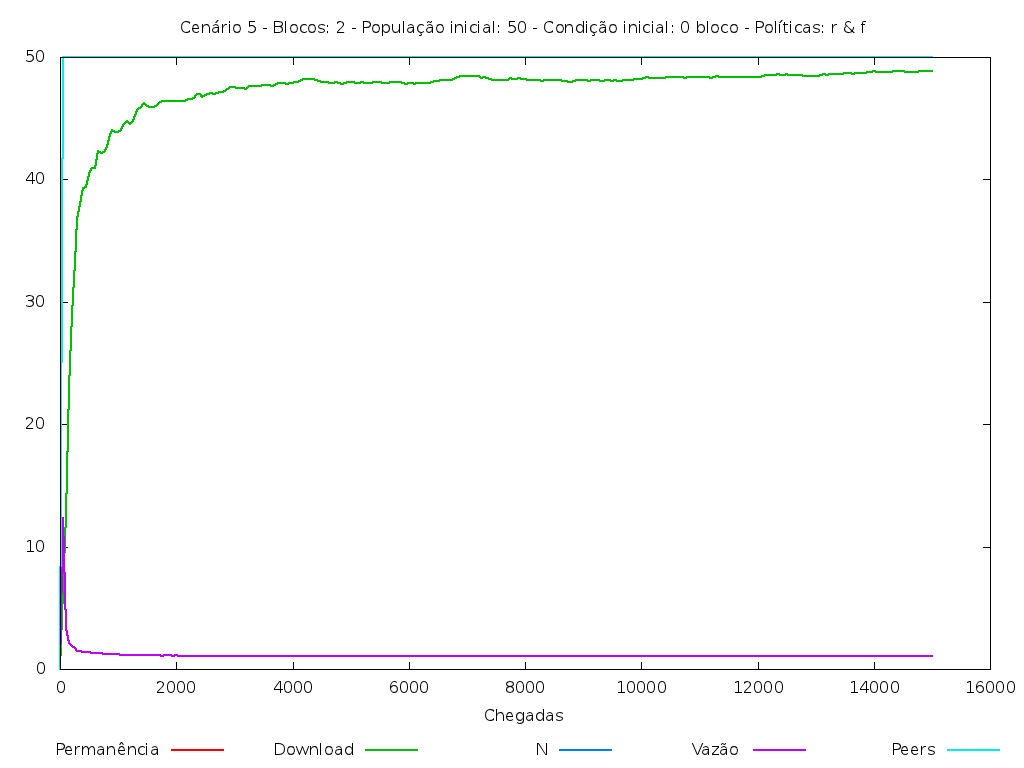
\includegraphics[scale = 0.33]{./graficos/condicaoInicial/03.png}
\end{figure}

\begin{figure}
	\caption{Visualização da fase transiente com política \textit{Random peer / Rarest first piece} e todos os peers iniciando com 1 bloco}
	\label{figCI1rf}
	\includegraphics[scale = 0.33]{./graficos/condicaoInicial/04.png}
\end{figure}

\clearpage
\pagebreak

\section{Conclusão}

Com base nos dados coletados, pudemos concluir que a presença de seeds no sistema tem um grande efeito sobre a escalabilidade do sistema. Além disso, pudemos perceber que aumentar o número de blocos também tem um efeito positivo na vazão do mesmo. Estas observações nos levam a compreender melhor os sistemas \textit{peer-to-peer} que utilizamos com frequência na internet de hoje em dia.

Entendemos que o modelo proposto pelo trabalho é bastante simplificado, mas acreditamos que as observações e dados aqui expostos têm grande valia para a compreensão total da realidade. A tarefa foi, portanto, bastante enriquecedora.

Uma grande motivação ao longo do desenvolvimento do trabalho foi a possibilidade de observar na prática os resultados teóricos estudados no decorrer do período. Toda a teoria ganha uma nova cara quando aplicada e isto foi uma das coisas que mais nos despertou o interesse.

\pagebreak

\end{document}
